\chapter{Project Deliverables}
\label{ch:projectdeliverables}
\section{Tasks and Responsibilities}
Stephen’s responsibilities were researching the feasibility of NAOs recognizing each other’s voices and to develop a detailed plan for the fusion of various mobile nets for recognition or navigation. After further testing of the NAO Robots, he was able to get the NAO Robots to recognize each other's voices and decided that the NAO robots are capable of performing the required tasks. Therefore, a custom mobilenet was not required. \par 

Zephaniah’s responsibilities were looking into NAO robot behavior to determine if the NAO Robots were able to overlap emotions and movement at the same time. After testing, the NAO Robots were able to detect multiple emotions at once but are not able to physically do multiple tasks at the same time. \par 

Seth’s responsibilities were to do research on all the sensors on the NAO Robot and to see how well they responded. Overall, all sensors on the NAO Robot were in good shape and were able to fully do the designed job they were intended for. \par 

Jacob’s responsibilities were to organize the shared drive and documents, troubleshoot issues with installing Choregraphe and NAOqi, help Stephen test the NAO robots’ capabilities, and develop a recognition module for Robot A. The recognition module still needs to be tested with other sensors other than just vision recognition. \par 

Overall, all team members worked together closely on all tasks and responsibilities. We worked together over Zoom meetings to complete all assigned tasks on blackboard on time and in-person meetings to test the NAO Robots functions.\par 


\section{Team Organization}

Together as a team we met every Wednesday at 2PM via Zoom along with Dr. Khan PhD student Megan, Dr. Khan assisted us when needed. Also, as a team we met in person one to two times a week to work on the NAO Robots. We kept a shared google drive open between all group members to complete assignments in a timely manner. Furthermore, the team has a group text chat to be able to get into contact with one another when needed. Here is a table \ref{tab:Past Meeting Schedule}of all our meetings so far this semester . Unless explicitly stated, it can be assumed that we also worked on that week’s assignment during the weekly meeting on Wednesdays. Every meeting lasted approximately an hour. \par 


\begin{table}
    \centering
    \caption{Past Meeting Schedule}
    \label{tab:Past Meeting Schedule}
    \scriptsize
    \begin{tabular}{| l | p{8cm} |}
      \hline
      \textbf{Meeting Date (Members)} & \textbf{Topics} \\
      \hline
      9/1/21 (Everyone)&Introduction to project. Determine whether we want to program real or virtual NAO robot. Relevant literature given.\\
      \hline
      9/8/21 (Everyone)&Discussed whether to go with the virtual or physical robot based upon Stephen’s findings. Decided to go with the real robots.\\
      \hline
      9/15/21 (Everyone)&Discussed overall project design. Made plans to meet day after.\\
      \hline
      9/16/2021 (Everyone except Megan)&Developed overall project design. Sent it to Megan for feedback.\\
      \hline
      9/22/21 (Everyone)&Split up project based upon everyone’s strengths and comfort levels with various modules.\\
      \hline
      9/29/21 (Everyone)&Discussed possible method to implement the recognition module. Creating our own network from scratch or using built-in functionality.\\
      \hline
      9/30/21 (Jacob, Stephen, Zeph)&Experimented with the NAO robots and tried to get familiar with the API. \\
      \hline
      10/6/21 morning (Everyone)&Further discussed the implementation of recognition modules either from scratch or using built-in functionality.\\
      \hline
      10/6/21 afternoon (Jacob and Stephen)&Built flow charts for the different recognition modules.\\
      \hline
      10/12/2021 (Everyone except Megan)&Used the flow charts to implement one large master plan for the entire project. Went very into depth on every module. Proposed multiple alternative designs and decided to perform feasibility tests to determine which design is the best.\\
      \hline
      10/13/21 (Everyone and Dr. Khan)&Met with Dr. Khan. Discussed our progress with him.  Decided to be more rigid and unforgiving with our deadlines. Decided that we have to implement and follow deadlines for ourselves.\\
      \hline
      10/14/21 (Jacob and Stephen)&Were able to get the NAO robots to recognize each others voice.\\
      \hline
      10/19/21 (Everyone)&Experimented with getting the NAO robots to recognize and classify each others eye color.\\
      \hline
      10/20/21 (Everyone)&Discussed environmental impacts of the NAO robots. Discussed making robot behaviors realistic \\
      \hline
      10/21/21 (Jacob, Stephen, Seth)&Were able to get the robots to recognize each other’s eye color. Decided on the following implementation for moods Red->Mad Green->Happy Blue->Neutral\\
      \hline

    \end{tabular}
  \end{table}


\section{Milestone Timeline}
All tasks we completed/will complete are listed in figure \ref{fig:Deadlines}. The start date is when we started or intend to start on a specific task and the end date is when we plan to finish the following task. \par 

\begin{figure}
    \centering
    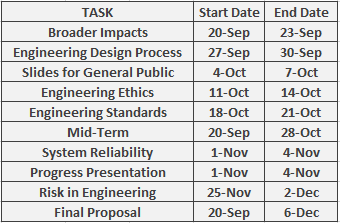
\includegraphics{chart}
    \caption{Assignment Deadlines}
    \label{fig:Deadlines}
  \end{figure}
